% !TeX root = ../main.tex

\chapter{BACS系统中的隐私保护}
\label{chap:privacy-design}

在第\ref{chap:bacs}中,我们介绍了基于区块链技术的ABAC访问控制系统。这一系统能增强现有访问控制系统的安全性,但引入联盟网络对用户信息进行共同管理,会导致联盟网络中任何节点都可以查看用户在系统中进行的授权信息和历史状态,带来用户隐私泄漏的风险。

第\ref{chap:privacy-survey}章对现有的隐私保护技术进行总结归纳。其中,zk-SNARK技术的优点在于生成的证明大小和验证证明的时间花销都是常数大小,缺点在于需要可信的初始化密码参数。因此,这一技术并不适用于公有链系统。而在BACS系统中,联盟链网络中节点可以通过安全多方计算技术共同参与密码参数的初始化过程,保障系统安全可信。同时,zk-SNARK技术提供常数级复杂度的验证可以保障BACS系统的实时性。

本章首先简要介绍zk-SNARK技术中的R1CS约束,QAP问题,同态加密三个主要步骤,然后介绍结合ABAC访问控制系统,区块链上授权的数据结构以及运用zk-SNARK技术进行隐私保护的方法。

\section{zk-SNARK技术}
\label{sec:zk-SNARK}

简明非交互式零知识证明(zk-SNARK,zero-knowledge Succinct Non-interactive ARguments of Knowledge)技术在非交互式零知识证明证明技术的基础之上进行优化,保持非交互性的同时,减少了证明大小,节省存储空间与验证时间。由于最终生成的证明转化为固定大小的多项式抽样验证,该技术的优点在于生成的证明大小为常数,验证该证明的时间花费也是常数。因此该技术能应用于区块链系统中事务合法性的证明和验证。缺点在于该技术需要可信的启动过程,通过一系列密码学参数来生成加密密钥和验证密钥,掌握这一类系列密码学参数即可伪造证明。该技术主要包含以下3个步骤:

\subsection{R1CS约束}

先将计算拆分为一阶线性约束等式(R1CS, Rank-1 Constraint System),这一过程类似编译器对高级语言程序进行处理到中间表示,每一步计算被转换为
$$s \cdot a * s \cdot b - s \cdot c == 0$$整个函数可能包含数百条甚至更多的R1CS约束,为了简化表示,也为了后面进一步简化,可以用矩阵的形式表达为
$$s \cdot A * s \cdot B - s \cdot C == 0$$

\subsection{QAP问题}

由于R1CS得到的矩阵形式中,每个矩阵包含若干列,对于每一行,可以通过拉格朗日插值公式构造特定函数fi(x)使得当x取值0到n的时候,刚好fi(x)值对应第i行第x列的数值。矩阵形式转换为多项式形式。

$$s \cdot A(x) * s \cdot B(x) - s \cdot C(x) == 0, \forall x = 1, ... , n$$

令$Z(x) = (x-1)(x-2)...(x-n)$,由多项式零点的性质可得s \cdot A(x) * s \cdot B(x) - s \cdot C(x)被$Z(x)$整除,即
$$s \cdot A(x) * s \cdot B(x) - s \cdot C(x) == Z(x)*H(x)$$ 对任意$x$成立

因此我们只需要验证该多项式等式是否即可,但由于多项式参数个数与约束数量相等,目前的验证未能节省时间。为了简化验证复杂度,因为该多项式在任意点都成立,因此通过验证一个特殊点,能以较大概率验证该多项式是否为0。因为2n次的多项式最多有2n个零点,证明者在不知道该特殊点的情况下伪造证明的概率约等于0。

\subsection{同态加密}

将计算的验证转换为对多项式等式的验证,并通过对点的抽样计算完成对整个多项式等式正确性的检验。基于椭圆曲线的双线性对性质隐藏用于计算的真实输入,包括证明者给定的隐私输入,以及验证者使用的特殊点。利用可信创始方初始化阶段生成的参数实现零知识证明.这一过程利用同态加密的加法同态性以及椭圆曲线的双线性对函数。验证者首先对特殊点t,生成t的次方加密后的值如下
$$E(1),E(t), E(t^2), E(t^3),..., E(t^n)$$

证明者可以通过这一系列参数计算出$E(A(t)),E(B(t)),E(C(t)),E(H(t))$。验证者为了验证$A(t)*B(t)-C(t) = Z(t)*H(t)$成立,只需要验证$E(A(t))*E(B(t))-E(C(t)) = E(Z(t))*E(H(t))$成立即可。这一证明可以隐藏证明者的特定输入$s$。

在访问控制系统中,存在资源服务器作为可信的启动方,独立生成初始密码学参数,不用担心其他人获取这些参数伪造证明。用户只需要根据资源服务器提供的加密密钥,以及自己的账户信息生成凭证,该凭证隐藏用户状态等部分敏感输入信息。资源服务器通过验证该凭证即可判断用户是否有权限执行提交的操作申请,并进行正确回应。具体设计将在第二部分介绍。

\section{BACS系统中的隐私保护设计}

在第\ref{chap:bacs}章中,我们提出了基于区块链技术的访问控制系统BACS,该系统中的授权数据结构和访问请求数据结构如图\ref{fig:data-structure}所示。其中,关键隐私信息为相关地址、授权属性、操作对象、操作类型等。该方案采用私钥签名作为来源凭证,在提供身份证明的同时暴露用户隐私信息。因此,本节将介绍采用zk-SNARK技术隐藏授权和访问中的关键信息。

\begin{figure}[ht]
  \centering%
  \subcaptionbox{授权信息数据结构\label{fig:auth-data}}
    {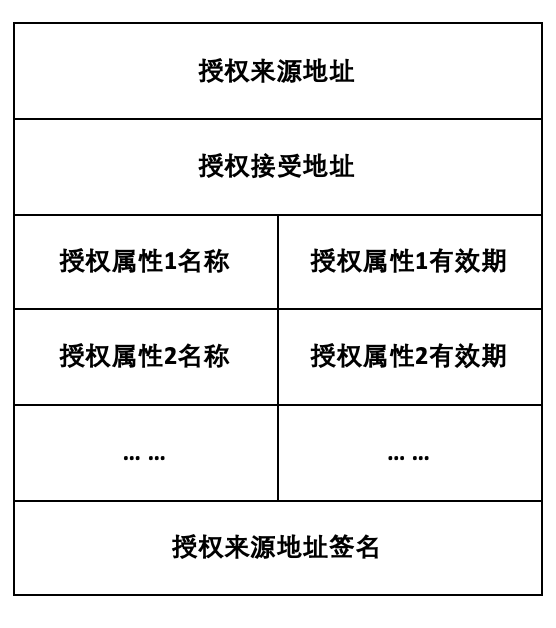
\includegraphics[width=6cm]{figures/auth-data.pdf}}%
  \hspace{4em}%
  \subcaptionbox{访问信息数据结构\label{fig:op-data}}
      {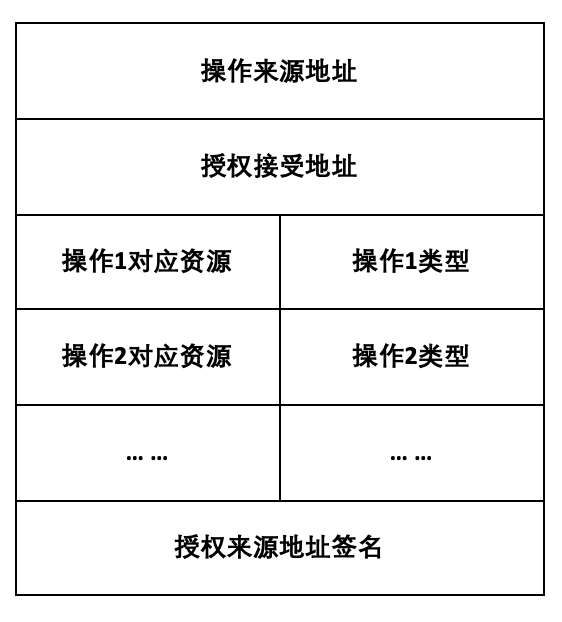
\includegraphics[width=6cm]{figures/op-data.pdf}}
  \caption{授权信息与访问信息数据结构}
  \label{fig:data-structure}
\end{figure}

\subsection{授权信息隐私保护}

对于授权数据,主要保护授权来源、授权对象和授权属性列表。首先设计统一的授权处理算法,该算法包含所有授权前后的状态的转换以及验证的操作。具体细节在算法\ref{alg:authVerify}中进行介绍。

 \begin{algorithm}
 \floatname{algorithm}{Algorithm}
 \caption{授权验证}\label{alg:authVerify}
   \begin{algorithmic}[!htbp]
   \renewcommand{\algorithmicrequire}{\textbf{Input:}}
   \renewcommand{\algorithmicensure}{\textbf{Output:}}
   \REQUIRE $Authorization$
   \ENSURE  $Verification$
    \STATE $Sender$, $Receiptor$, $Attributes$, $nonce$, $Signature \gets Parse(Authorization)$
    \STATE $AuthorizationHash \gets Hash(Authorizaton)$
    \IF {$CheckSignature(Sender, Hash, Signature) \ne true$}
      \RETURN $false$
    \ENDIF
    \STATE $SenderState \gets GetStateFromAddress(Sender)$
    \IF {$nonce < SenderState.nonce$}
      \RETURN $false$
    \ENDIF
    \FOR {$each Attribute \in Attributes$}
      \IF {$SenderState.VerifyAttribute(Attribute) \ne true$}
        \RETURN $false$
      \ENDIF
    \ENDFOR
    \STATE AddAuthorizationToPool(Authorization)
   \RETURN $true$
   \end{algorithmic}
 \end{algorithm}

利用zk-SNARK技术,可以将该算法转换为同态加密下对多项式的验证,并且利用起始阶段生成的证明密钥和验证密钥,授权用户可以对合法的输入给出可信证明,联盟网络中节点在收到该证明后可以在常数时间复杂度内进行验证,并对状态进行修改。

\subsection{操作信息隐私保护}

对于操作数据,与授权数据的不同之处在于,资源服务器必须针对资源进行正确的操作,因此必须知晓操作对象和操作类型,而需要保护操作来源。算法\ref{alg:authVerify}介绍了对操作进行验证的具体步骤。

 \begin{algorithm}
 \floatname{algorithm}{Algorithm}
 \caption{验证操作}
   \begin{algorithmic}[H]\label{alg:opVerify}
   \renewcommand{\algorithmicrequire}{\textbf{Input:}}
   \renewcommand{\algorithmicensure}{\textbf{Output:}}
   \REQUIRE $Operation$
   \ENSURE  $Verification$
    \STATE $Sender$, $OpCode$, $Obj$, $nonce$, $Timestamp$, $Signature \gets Parse(Operation)$
    \STATE $OperationHash \gets Hash(Operation)$
    \IF {$CheckSignature(Sender, Hash, Signature) \ne true$}
      \RETURN $false$
    \ENDIF
    \STATE $SenderState \gets GetStateFromAddress(Sender)$
    \IF {$nonce < SenderState.nonce$}
      \RETURN $false$
    \ENDIF
    \STATE$SubAttributes \gets GetAttrFromAddress(Sender)$
    \STATE$ObjAttributes \gets GetAttrFromObject(Obj)$
    \STATE$OpAttributes \gets GetAttrFromOpCode(OpCode)$
    \STATE$EnvAttributes \gets Timestamp$
    \FOR {$each Policy \in Policies do$}
      \IF {$Policy.Match$($SubAttributes$, $ObjAttributes$, $OpAttributes$, $EnvAttributes$) = $true$}
        \RETURN $true$
      \ENDIF
    \ENDFOR
   \RETURN $false$
   \end{algorithmic}
 \end{algorithm}

在这一算法中,输入的Sender,nonce,Timestamp和Signature信息为隐藏字段,构造在节\ref{sec:zk-SNARK}介绍的$s$中,而OpCode和Obj字段为公开字段,资源服务器根据存储的属性访问控制列表对操作进行验证后得出结论。

